\begin{solution}
    \begin{enumerate}[label = \Alph*)]
        \item After combining the industry portfolios dataset with the FF factors, the remaining dataset contains 288 monthly excess returns for 4674 mutual funds. Calculating the principal components for \(k = 1, \dots, 5\), Figure~\ref{fig:ck_explained_var} plots the explained variance ratio for each of these portfolios. From this figure, we see that the amount of variance explained by the first factors is quite low compared to the previous exercise. 
        \begin{figure}[!htbp]
            \begin{small}
                \begin{center}
                    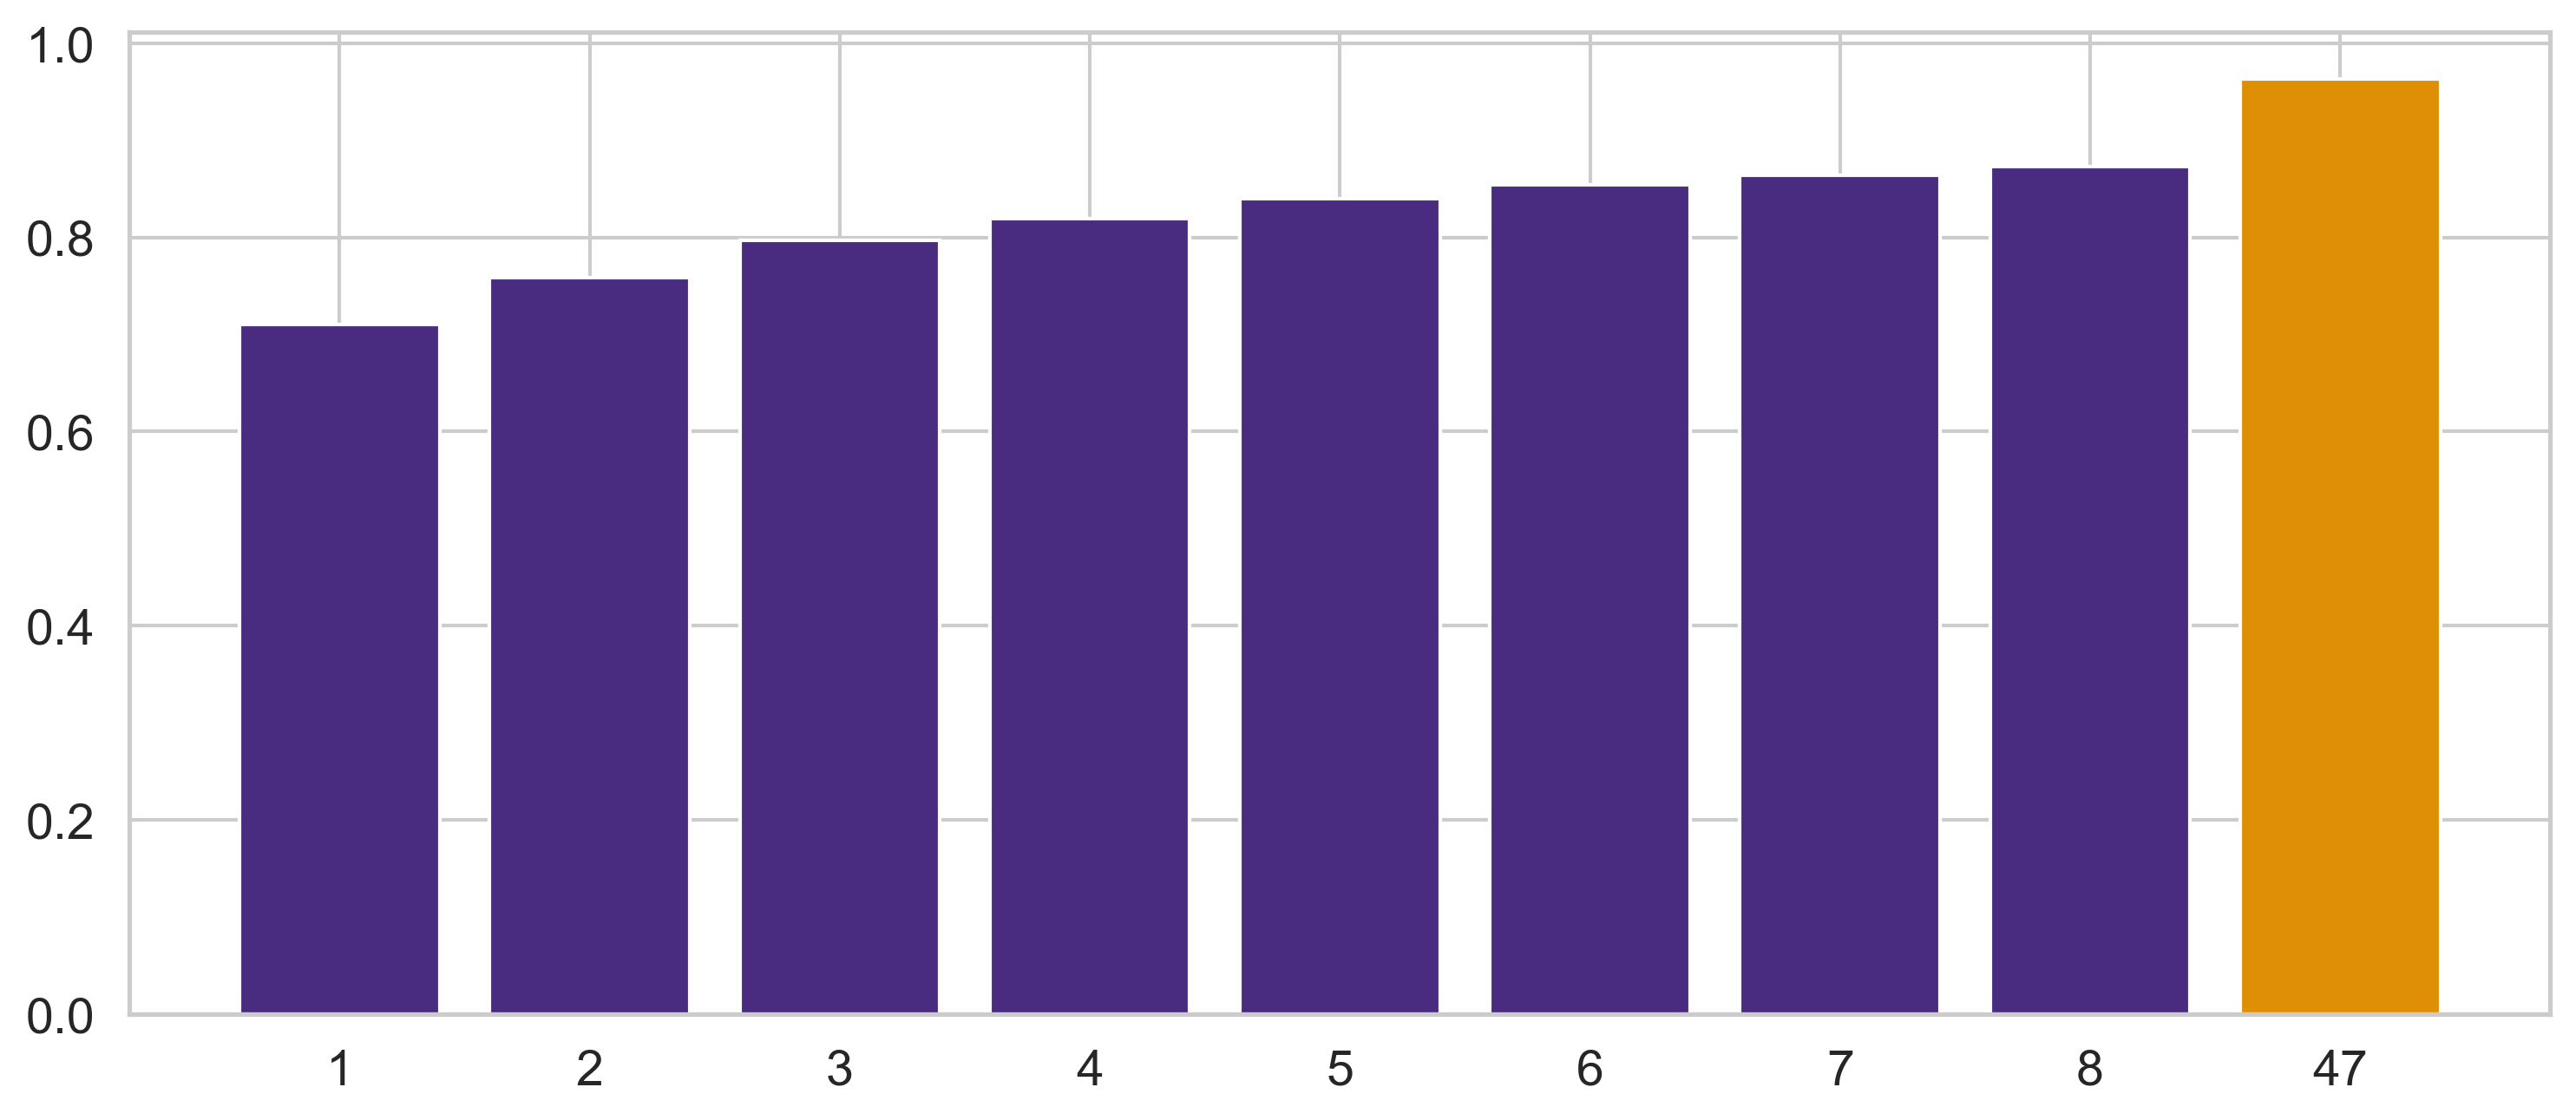
\includegraphics[width=0.8\textwidth]{ck_explained_variance.png}
                \end{center}
                \caption{Explained Variance Ratio for the set of \(k\) components}
                \label{fig:ck_explained_var}
            \end{small}
        \end{figure}
        The correlation between the 6 principal components and the FF factors is depicted in Figure~\ref{fig:ck_pca_ff}. The first principal component still mostly captures the market portfolio. However, we see a greater influence of the momentum factors in each of the components. 
        The second PC captures other important factors such as HML, RMW and CMA. Finally, SMB is mostly correlated with PC4, PC5 and PC6.
        \begin{figure}[!htbp]
            \begin{small}
                \begin{center}
                    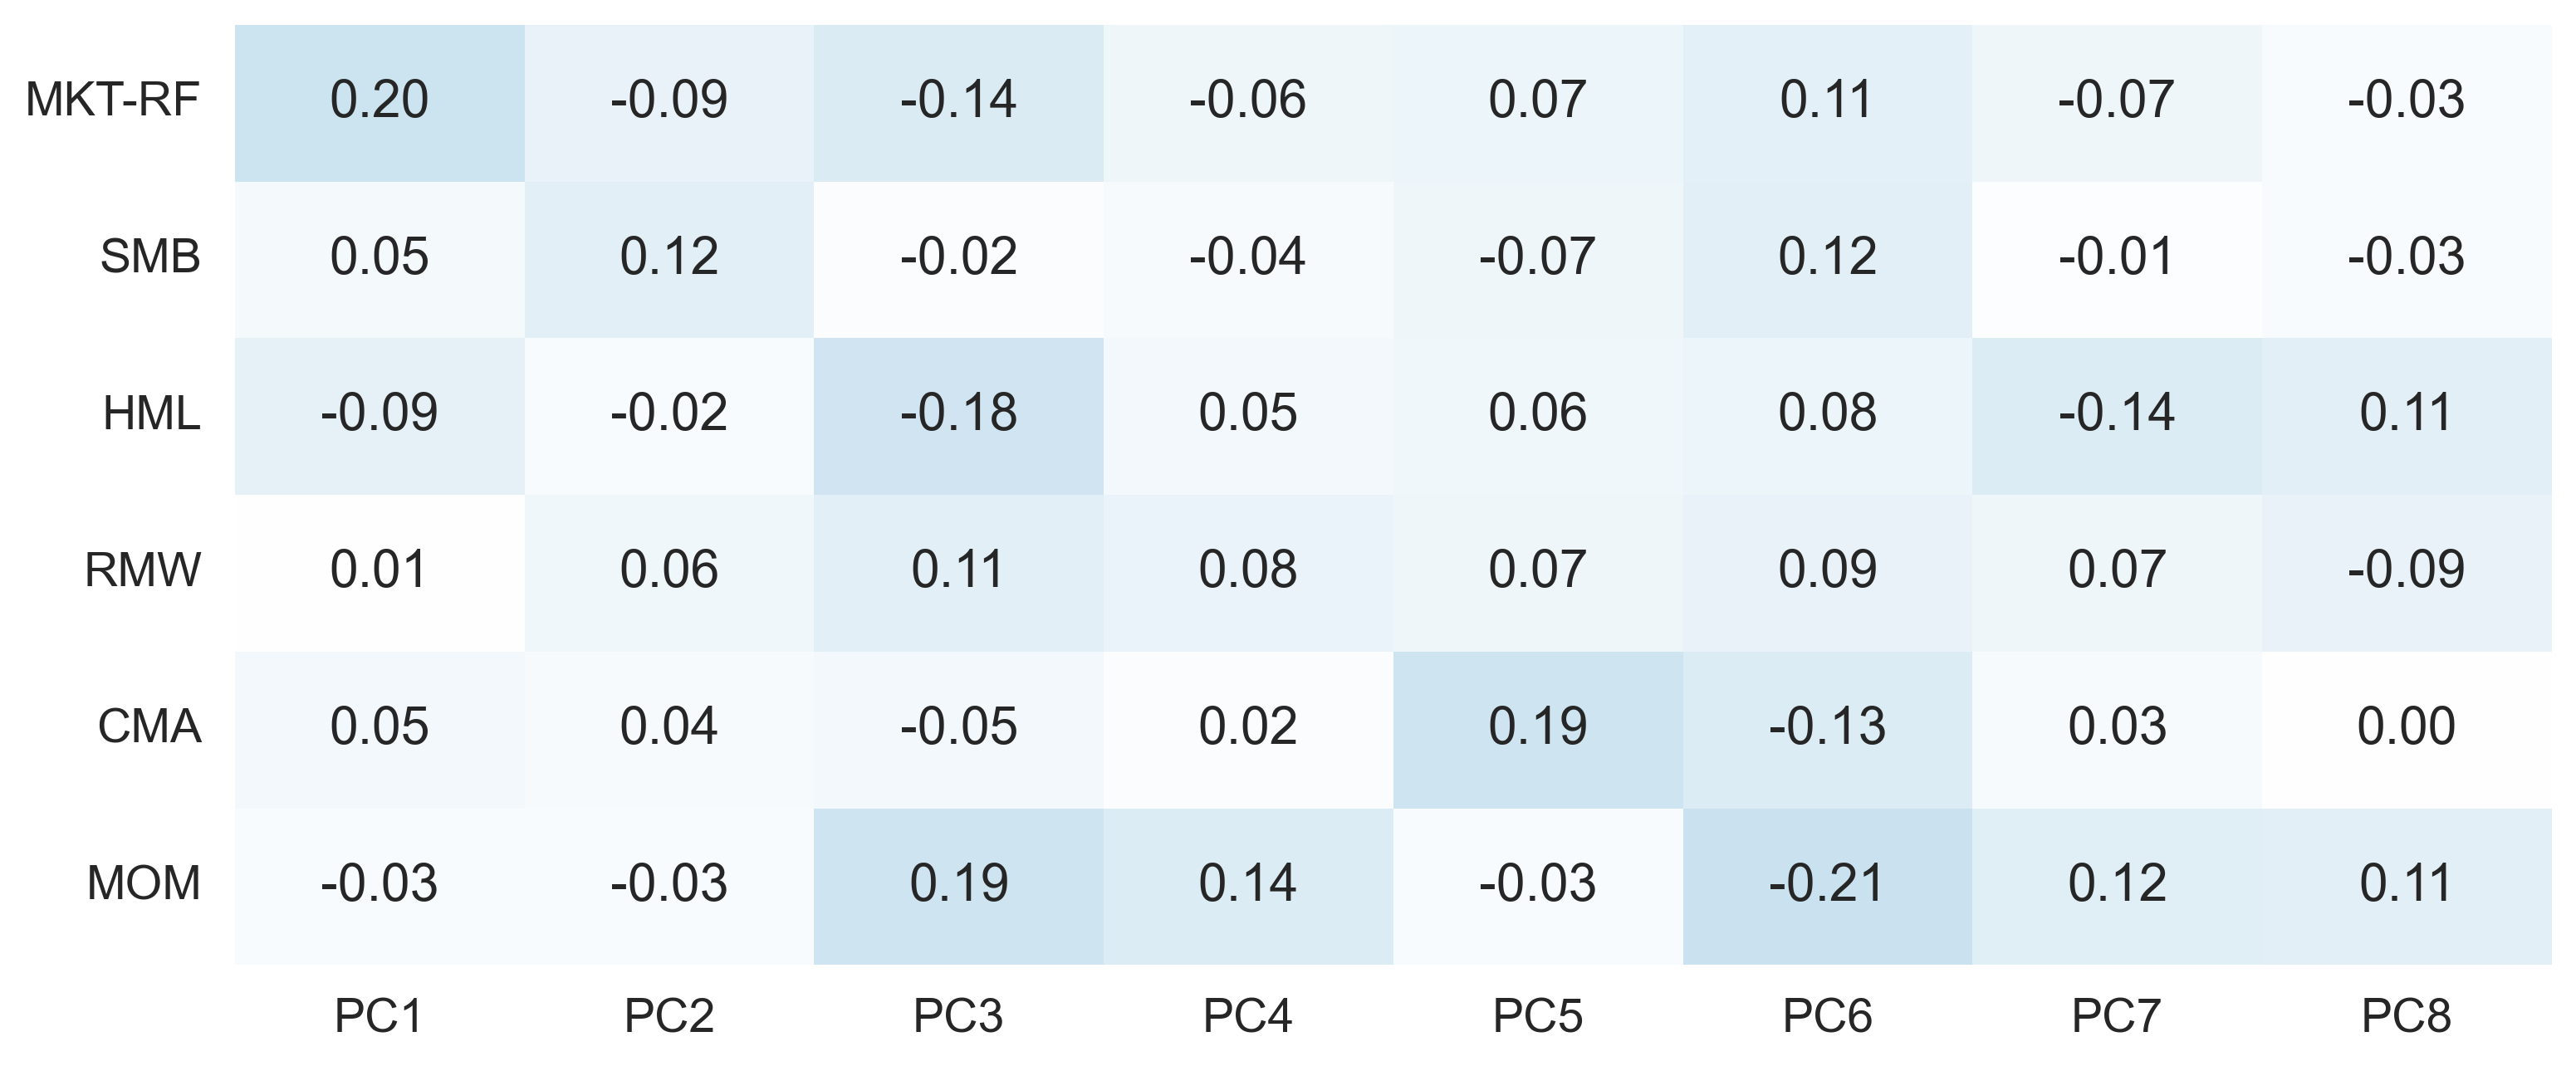
\includegraphics[width=0.8\textwidth]{ck_pca_ff_corr.png}
                \end{center}
                \caption{Correlation between Principal Components and FF Factors}
                \label{fig:ck_pca_ff}
            \end{small}
        \end{figure}
        
    \item I use the \citet{connor1993test} to find the optimal number of factors. Using the entire sample, only 1 factor is required to explain a large portion of the variance of the 4674 mutual funds. Figure~\ref{fig:ck_explained_var} shows the explained variance ratio for the first 6 components and the optimal number. We can see that there is not a significant increase in the explained variance ratio compared to the model with 6 components as the first factor already explains most of the variance.
    
    \item Using the optimal number of factors, I estimate the Appraisal Ratio for each fund in the sample and calculate the critical values of \eqref{eq:appraisal_distribution}. The distribution is shown in Figure~\ref{fig:appraisal_dist}. We see that there is a significant number of funds outperforming the market in the overall sample. A total of 1271 funds have a positive and significant appraisal ratio when using the asymptotic distribution.
    
    \begin{figure}[!htbp]
        \begin{small}
            \begin{center}
                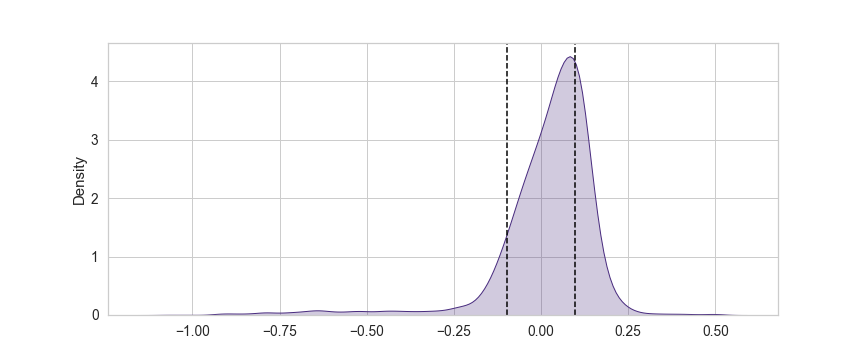
\includegraphics[width=0.8\textwidth]{appraisal_ratio_dist.png}
            \end{center}
            \caption{Distribution of Appraisal Ratio}
            \label{fig:appraisal_dist}
        \end{small}
    \end{figure}
    
    \item Using data for over 20 years of returns, it is hard to expect that the sensitivity of funds to each factor would have stayed the same. Different macroeconomic conditions, for example, can affect the strategies and performances of each fund. To account for this, I estimate the same model using 2 halves of the sample. The first subsample contains data from 2000 to 2011, while the second spans from 2012 to 2023. I run the model for each subsample and calculate the optimal value of factors. Unlike in the overall sample, the subsamples indicated an optimal number of 1 and 6 factors respectively, smaller than the full sample. Figure~\ref{fig:ck_appraisal_sub} shows the distribution of the Appraisal Ratio for both subsamples. As we see, these ratios tend to be higher in the first subsample, compared to the second. A total of 1638 (\(\approx 35\%\)s) of funds outperformed in the first half and 980 (\(\approx 21\%\)) in the second half and only a 498 (\(\approx 10\%\)) of funds did well in both samples. This exhibits the difficulty in maintaining a good strategy throughout different market conditions.
    
    \begin{figure}[!htbp]
        \begin{small}
            \begin{center}
                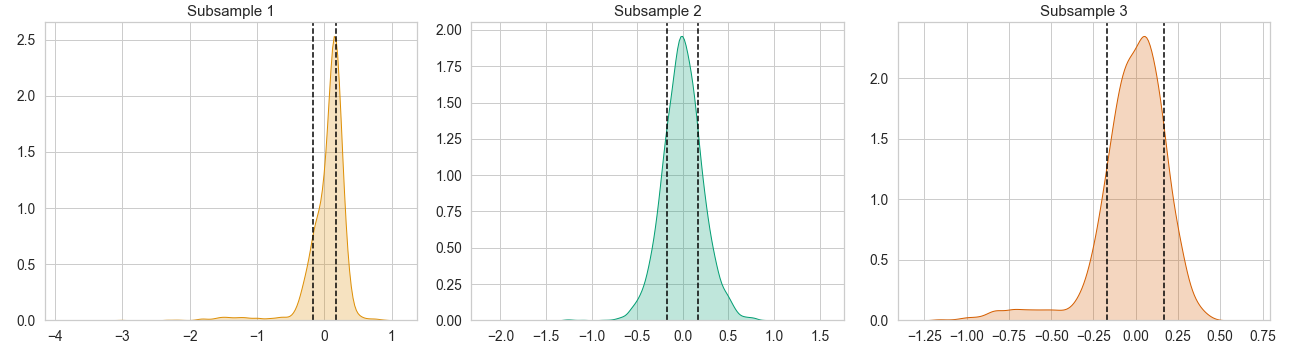
\includegraphics[width=0.8\textwidth]{apprisal_ratio_sub.png}
            \end{center}
            \caption{Distribution of Appraisal Ratio for Subsamples}
            \label{fig:ck_appraisal_sub}
        \end{small}
    \end{figure}
    
\end{enumerate}
\end{solution}